\section{Hyper Content}
	In this section we describe the algorithm we created to show synchronized interactive content to clients.


	\subsection{Content creation}

	In order to create content the user has the option to write simple movie captions without writing any code, otherwise, as mentioned before, it can write \ac{HTML}, \ac{CSS} and \emph{JavaScript}. The definition of the content's starting and ending time by the user it's not an easy task. Defining the content's time to appear in real-time would require a previous user plan. Otherwise the user could make a speech and add the content for later reproduction.

	Figure \ref{fig:creation} shows the user interface for creating interactive hyper content manually.

	\begin{figure}[H]
		\centering
		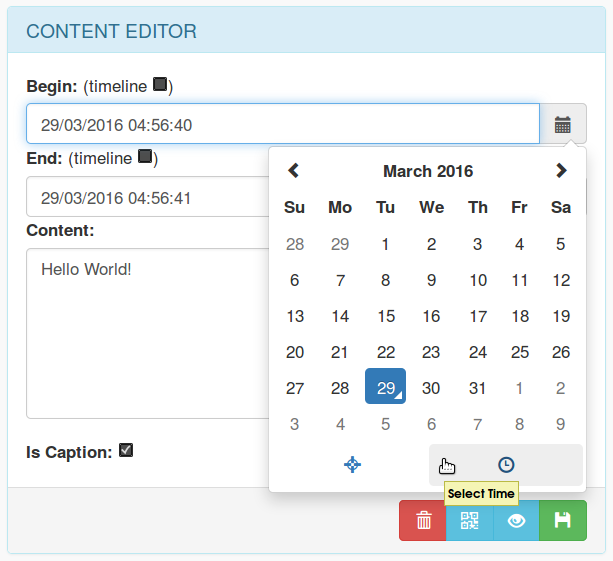
\includegraphics[width=0.6\textwidth]{figures/edition.png}
		\caption{Manual content creation}
		\label{fig:creation}
	\end{figure}


	Listing \ref{lst:createcontent} shows the structure of the content created by one user.

\begin{minipage}{\linewidth}
\begin{lstlisting}[caption={Exampe of content created by one user},label={lst:createcontent},language=json]
{
	"cmd":"createContent",
	"start":"2016-03-29T03:56:40.000Z",
	"end":"2016-03-29T03:56:41.000Z",
	"content":"<h1>Hello</h1>"
}
\end{lstlisting}
\end{minipage}
	In order to help the content creator to show and synchronize its content in real-time we allow the user to encode its content into \emph{QR codes} and show it to the camera in real time.

	\ac{KMS} lets registering event handlers for \emph{QR code} detection. The component that detects \emph{QR codes} on \ac{KMS} is called periodically and fires the handlers with the decoded content. This mechanism does not detect if the \emph{QR code} enters or leaves the screen. We had to implement our own mechanism for detecting those events.

	Each user session in the server maintains a map with the contents that are present on the screen. In order to apply our algorithm more efficiently we calculate the content's hash through the \emph{md5} method.

	If the hash is not present in the map it means the \emph{QR code} was entering the screen, we add that hash to the map and associate the current time to it, all the users are notified to watch that content in real-time. By doing an analogy to the \emph{Nyquist} theorem we know that if the same \emph{QR code} is not detected after a time bigger then two periods we can conclude that the \emph{QR code} leaved the screen and we add the correspondent content into our database. Listing \ref{lst:pseudo_qrcode} shows the pseudo code for \emph{QR code} leaving detection.

\begin{minipage}[!htb]{\linewidth}
\begin{lstlisting}[caption={Pseudo code for QR code leaving detection},label={lst:pseudo_qrcode},language=JavaScript]
var ongoingCodesMap = {};
function onCodeFound(content) {
	var startingTime = getCurrentTime() - getUserOffset();
	var hash = md5(content);
	if(ongoingCodesMap[hash] == null){
		sendQRCodeToEditingUser(hash,content);
	}
	ongoingCodesMap[hash] = startingTime;
	waitTwoSeconds(); // onCodeFound() may be called from other threads
	var newestTime = ongoingCodesMap[hash]; 
	if(newestTime == startingTime){
		var endingTime = getCurrentTime() - getUserOffset();
		ongoingCodesMap[hash] = null; 
		sendQRCodeToEditingUser(hash,null); // remove from UI
		insertContentIntoDatabase(startingTime,endingTime,content);
		sendContentToUsers(startingTime,endingTime,content);
	}
}
\end{lstlisting}
\end{minipage}


	Our main content synchronization mechanism is time based but with some programming knowledge it is possible to insert \emph{JavaScript} code that fires events on user interaction. For example, after a teacher's lecture, it is possible to show a quiz to the users in order to understand what they learned and then submit the data to the server for further analysis.


	\subsection{Interactive media synchronization}

	In our solution content is represented as simple text that can contain \ac{HTML}, \ac{CSS} or even \emph{JavaScript}, this content is displayed on defined intervals of time.

	Multiple contents can be displayed at the same time, in order to achieve that, we define layers above the video with the same size. Each layer is associated to the content.

	We have taken into account that the amount of content tends to grow with time and the user should only have access to a subset of content instead all of them, which would be very inefficient.

	The content to display for each user depends on the user's position on the time-line, this position is given by an offset between the current time and the navigated time. If the user is watching the content in real-time this offset is constant so there is no need to synchronize this value.

	Each content is divided into two components, the \emph{start} and the \emph{end} which are sent to users. The \emph{start} component contains a time stamp, the content identification number and the content itself in form of text. The \emph{end} component only contains the time stamp and the content identification number. 

	The content to return is given by the union of two content subsets:
	\begin{itemize}
		\item The intersection of the content interval and user's time.
		\item A subset of contents which starting time is immediately following the user's time.
	\end{itemize}

	The second subset is used for predicting which content the user will watch and avoid requests during its events.

	The content description messages that are sent to each user contains the constant itself on the form of a list of events and an attribute that specifies if the server has more content to return.

	Listing \ref{lst:sentcontent} shows the structure of the content sent to users.

\begin{minipage}{\linewidth}
\begin{lstlisting}[caption={Exampe of content sent to users},label={lst:sentcontent},language=json]
{
	"cmd":"content",
	"data":[{
			"id":"56f9fd1aa986c615fab43d69",
			"time":"2016-03-29T03:56:40.000Z",
			"type":"start",
			"content":"<h1>Hello</h1>"
		},{
			"id":"56f9fd1aa986c615fab43d69",
			"time":"2016-03-29T03:56:41.000Z",
			"type":"end"
		}
	],
	"more":false
}
\end{lstlisting}
\end{minipage}

	When a user enters the conference room, immediately after the \emph{WebSocket} creation the server sends him the current content.

	The user receives the content, sorts all components by time and creates a set of events. All the events before the user's time are rendered and removed from the set of events. A timer is scheduled for the first component on the event set and the process repeats while the set is not empty.

	If the set is empty, there two options, if the server contained more content a new request for content is made and the process starts from the beginning, namely the server sends the correspondent content again. If the server has no more content the process is stopped until it sends more.

	The users will receive their contents from the server on five different situations:

	\begin{itemize}
		\item Conference room entrance (advertised by server).
		\item Set of events empty and server has more content (client requested).
		\item Content is created (advertised by server).
		\item Content is removed (advertised by server).
		\item User navigates to different point in time (client requested).
	\end{itemize}



	Listing \ref{lst:pseudo_render} presents the pseudo code for our content scheduler.

\begin{minipage}[!htb]{\linewidth}
\begin{lstlisting}[caption={Pseudo code for hyper content scheduler},label={lst:pseudo_render},language=JavaScript]
function scheduleContent() {
    var navigatedTime = getCurrentTime() - getUserOffset();
    while ( hasLocalEvents() ) {
        if ( firstEventIsOlderThanNavigatedTime() ) {
            if ( firstEventIsStart() ) {
            	addHtmlLayer(event);
            } else {
            	removeHtmlLayer(event);
            }
            removeFirstEvent();
        } else {
            break;
        }
    }
    if ( hasNoLocalEvents() ) {
    	return;	// nothing to do
    } 
    if ( hasNoStartEvents() && serverHasMoreContent() ) { 
       	requestContentFromServer(navigatedTime);
    } else {
        waitUntilNextEvent();
        scheduleContent();
    }
}
\end{lstlisting}
\end{minipage}

	\subsection{Security Concerns}

	Our solution is flexible on what kind of interactions are possible to the users in real time but allowing users to write \emph{JavaScript} that is executed on the other users browser would attackers to misuse their resources and access to critical information.

	We could solve this problem easily by escaping any \emph{script} tag present on the content, but we would sacrifice the kind of interactions that are possible. 

	By not allowing \emph{JavaScript} we would need to implement all actions a priori and fire them when a type of message is received. We decided to ignore the security vulnerabilities that are exposed by evaluating \emph{JavaScript} because in order to offer the same interactions we would have to do an exhaustive functional requirements gathering.

	Another way to solve this problem, which is not within the goals of this thesis, is to analyze the \emph{JavaScript} code and detect if it is malicious.

	\subsection{Time Manipulation}

	We have used \emph{vis.js} to display out time-line. This library was created for content navigation through time, but it was not designed to be always moving automatically, we have created a background timer that performs the animation of moving the window of time bounds and user navigated time marker.

	Figure \ref{fig:timeline} shows the the graphic appearance of our interactive time-line, in order to navigate through time the user must drag and drop the time-line horizontally, when the user drops the time-line an event handler is called with the new user's time offset which will be used to send a message to the server in order to choose the correspondent content to display. 

	\begin{figure}[!htb]
		\centering
		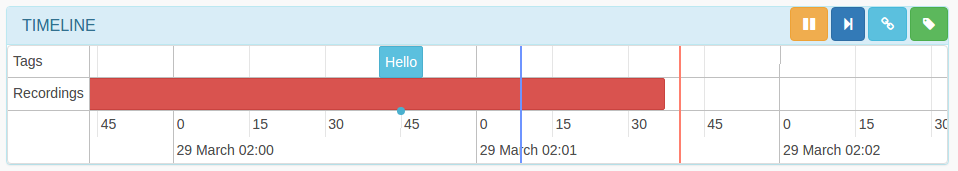
\includegraphics[width=\textwidth]{figures/timeline.png}
		\caption{Interactive time-line}
		\label{fig:timeline}
	\end{figure}

	We have noticed the server time being different from client time and this created graphic inconsistencies such as showing existing recorded blocks of movie in the future. To solve this problem the server sends its time to client immediately after the \emph{webSocket} creation, we synchronize the time-line with the server and although it may exist a small error due to network transmission time the graphical error is negligible. 


	\subsection{Time annotations creation}

	Time annotations are simpler way save points in time and share them with other users. When a user enters in a conference room the server sends all annotations so they can be displayed directly into the user time-line. Each time annotation is created all users are advertised so they can update their interfaces.

	Figure \ref{fig:annotation} shows the creation and placement of annotations on the time-line, to save the annotation the user must click on the floppy icon in order to save it and advertise the conference participants. 

	\begin{figure}[!htb]
		\centering
		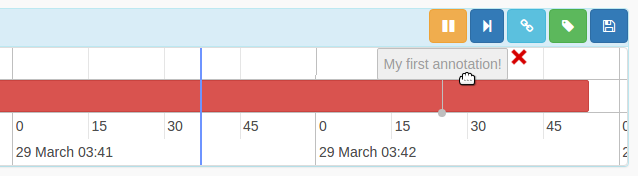
\includegraphics[width=0.7\textwidth]{figures/annotation.png}
		\caption{Creating a time annotation}
		\label{fig:annotation}
	\end{figure}

	Besides the ability to create tags it is also possible to create time hyper-links, see figure \ref{fig:timelink}, that can be sent to other users externally so they can navigate directly to the content when entering in the conference room.


	\begin{figure}[!htb]
		\centering
		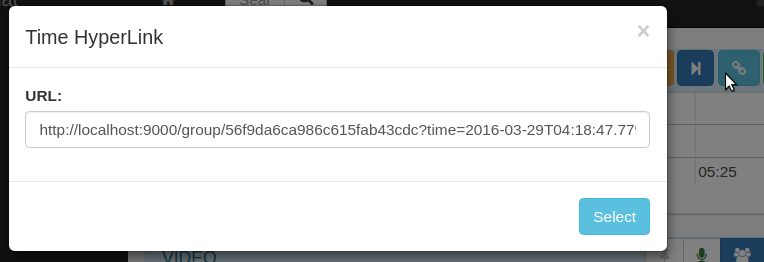
\includegraphics[width=0.8\textwidth]{figures/timelink.png}
		\caption{Time link creation}
		\label{fig:timelink}
	\end{figure}


	\subsection{Content Search}

	Users can easily search for annotations and contents and travel to their correspondent times. In the case of hyper content after handling the result from database we ignore \ac{HTML} tags, extract the text with \emph{Jsoup}\footnote{\url{http://jsoup.org/} (Accessed 21 March 2016)} and apply the query again. We extract the text from \ac{HTML} because accidentally searching for text contained in \ac{HTML} tags would lead to incorrect results.

	Figure \ref{fig:search} shows how the search results are displayed to the user. Each result entry contains an icon specifying the type of result (hyper content, time annotation, ...).




\begin{figure}[!htb]
\centering
\begin{minipage}[b]{0.55\linewidth}
\centering

		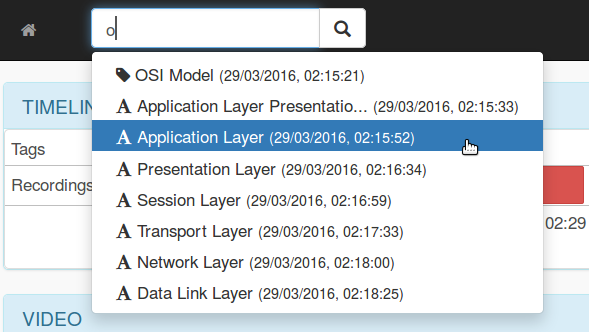
\includegraphics[width=\textwidth]{figures/search.png}
	      a) Result list
\label{fig:minipage1}
\end{minipage}
\quad
\begin{minipage}[b]{0.40\linewidth}
		\centering

		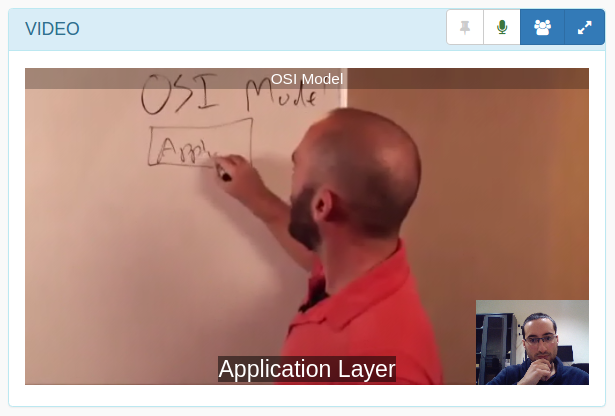
\includegraphics[width=\textwidth]{figures/search2.png}
	       b) Selected result
\label{fig:minipage2}
\end{minipage}

		\caption{Example of search results}
		\label{fig:search}
\end{figure}


	\subsection{Switching views}

		We provide a way for users to select the composite view of the conference room or the video shared by a particular user device as it can be seen on figure \ref{fig:devices}. 

		In order to maintain a list of available user devices that can be played at the navigated time if a user plays or ends playing a block of recorded video it obtains at the same time a list of all devices available for each user at that time.

		On the other hand, if a user changes to real time, the list of devices is extracted from the set of \emph{webSockets} that are associated to the respective conference room. This list of devices is also sent to the users that are also in real time mode whenever a new user enters or leaves the conference room.

	\begin{figure}[!htb]
		\centering
		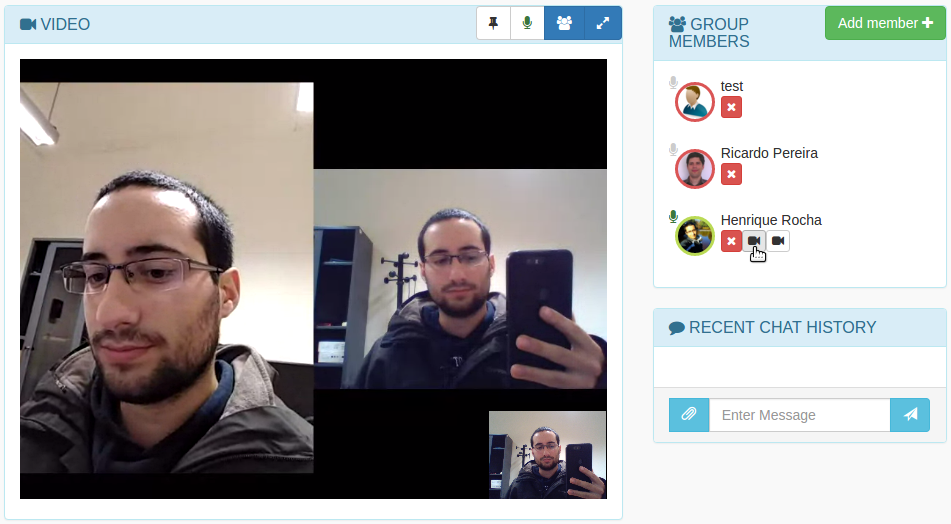
\includegraphics[width=0.8\textwidth]{figures/devices.png}
		\caption{Multiple devices per user}
		\label{fig:devices}
	\end{figure}

		We also provide an automatic mechanism for switching the view to the current speaker. With respect to sound analysis, the sound samples are analyzed on the client side through the web audio \ac{API}.

		Our speech detector is straightforward, we could perform a spectral analysis in order to understand if the analyzed sound contains frequencies in the range of the human voice but instead we just capture sound samples in real time and calculate the maximum sound amplitude. If a sound sample has an amplitude bigger than a factor of the maximum amplitude (we have used an empirical value of 10\%) we say that the user is speaking and therefore we send a message to the server if the speaking state has changed. Subsequently, the server receives the user speaking state and sends it to the other users so they can request a different view.


\subsection{Non interactive media synchronization}
		By default each user receives the real time mixed video and audio of every users. As described on the previous section, users can switch the current view even for recorded media.

		Whenever a user changes the current viewed time, our server calculates which chunks to reproduce.

		In order to determine which chunks are going to be played we could find any chunk that matches the session id and intersects the given user time. Although this seems logical, we limit the size of the results to one and ignore the starting component of the recording chunk. As a consequence, we will obtain the recording chunk that ends after the playing time.

		The obtained chunk may or not intersect the given time, if it intersects than we immediately start playing the chunk, otherwise we know that the chunks starting time is after the playing time and we schedule the player to reproduce after a time duration given by the difference of the playing time and chunk starting time.

		In order to reduce the delay between switching parts we perform a query on the database for finding the next chunk to play while the selected media is playing. In order to find the next chunk we use the chunk that has a bigger id immediately after the playing chunk.

		In order to allow the users to watch an individual image and ear the audio of everyone, we are using two players, one for audio and another for video. 

		If a user leaves a conference room, it is expected that the sequence of played blocks ends. When a block is not found for a given \emph{webSocket} session we try to find a block for the same user and if not possible we try to play a composite recorded block, lastly, if every attempt fails we wait for the next interval the contains media.
